\subsection{Database connection}
Every time you will start \edacc you will be prompted to provide the connection data to the \mysql database you would like to work with. 
\begin{center}
	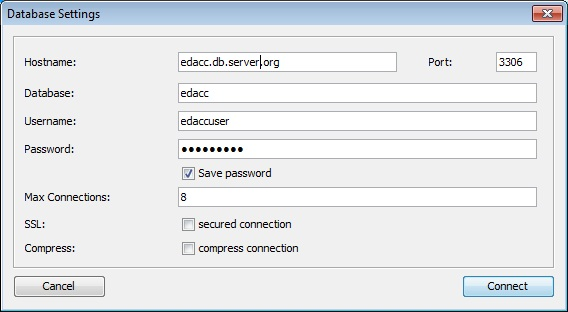
\includegraphics[width=1.00\textwidth]{snapshots/DBlogin.jpg}
\end{center}

\marginlabel{Host name / IP}In the connection dialog you have to provide the host name or the IP-address of your \mysql database. 

\marginlabel{Port}If you have configured the \mysql server to use an other port then the default \mysql port 3306, you can specify this in the \textbf{Port:} text field. 

\marginlabel{DB name} Further you also have to provide a valid database name and a user along with the corresponding password. 

\marginlabel{Save password} If you would like to save the password of this connections for further usage you can check the \textbf{Save password} check-box. \edacc will save the password for you in a configuration file. \attention The password is saved in plain text, so if other users have access to your private files they will be able to read the password from the configurtion file. 

\marginlabel{Max Connections} \edacc is a multi-threaded program and will use more than on connection to the database to speed up certain tasks. We recommend to allow up to 8 simultaneous database connections, but if you have restrictions on this number you can specify it in the \textbf{Max Connection:} text field. \todo Simon: wenn das weniger sind?

\marginlabel{SSL connections} If you are going to use \edacc to store trusted data we strongly recommend to enable a SSL connection by checking the \textbf{secured connection} check box. \todo Be aware that this kind of connection is only possible is the \mysql server is configured accordingly. 

\marginlabel{Compressed Connections} When working with \edacc through a slow network connection you might want to turn on compression by checking the \textbf{compress connection} check box. 

\marginlabel{Connect} After providing all the information you can connect to the \mysql server. 

\marginlabel{Create DB} When you connect the first time to a database \edacc will create for you all the needed tables. \todo Was passiert wenn man sich an einer falschen DB verbindet, die ein anderes Modell hat. Kann man das EDACC DB Modell neu erzeugen �ber einen bestehenden? 

\marginlabel{DB Model version} 
As \edacc is under full development and the database model may be extended to support new features, \edacc will check if the database model is compatible with the GUI version. Within this check we  differentiate between two cases:
\begin{enumerate}
	\item \ml{DB Model upgrade}The database model version is to old for the GUI. In this case \edacc will offer you the possibility to upgrade your database scheme to the latest version. \todo Werden da auch mehrere versionen �bersprungen? Sprich von version 0.1 auf 0.4?
	\item \ml{GUI update}The database model version is to new for the GUI. In this case you should update the GUI. You can do this by using the automatic update function of \edacc, which can be found under \textbf{Help $\rightarrow$ Check for Updates}. Another possibility is to download the latest release form the project site at \url{http://sourceforge.net/projects/edacc/}. 
\end{enumerate}